\documentclass{article}%[12pt, a4paper]{article}

\usepackage{ucs}
\usepackage[russian]{babel}
\usepackage{cmap}
\usepackage[utf8x]{inputenc}
\usepackage{amsthm}
\usepackage{amsmath}
\usepackage{amssymb}
\usepackage{graphicx}
\usepackage{float}
\usepackage{clrscode}
\usepackage{tocloft}
\usepackage[usenames]{color}
\usepackage[margin=20mm]{geometry}
\usepackage{sidecap}
\usepackage{url}
\usepackage{hyperref}

\frenchspacing



\begin{document}

\thispagestyle{empty}

\begin{frame}
  \maketitle
 \end{frame}

\setcounter{page}{1}

\section{Введение}
\subsection{Постановка задачи}

\begin{frame}
  \frametitle{Введение}
  \begin{defn}
     Восстановить машинное представление молекулы, утерянное при отрисовке
  \end{defn}
  \begin{center}
  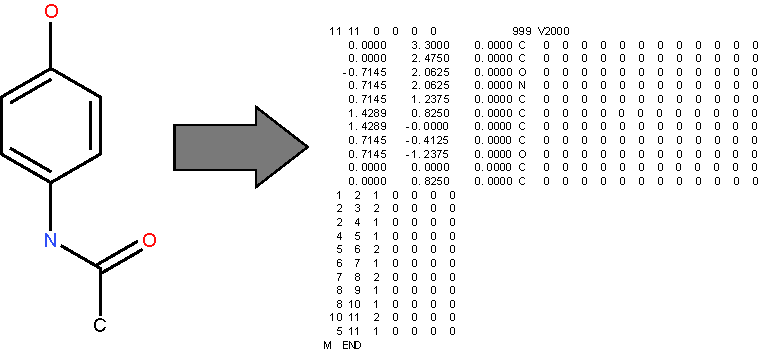
\includegraphics[scale=0.8]{media/parac.pdf}
  \end{center}
\end{frame}

\subsection{Возникновение задачи}

\begin{frame}
  \frametitle{Введение}
  \framesubtitle{Возникновение задачи: работа с публикациями}
  \begin{center}
    \href{run:media/demo.wmv}{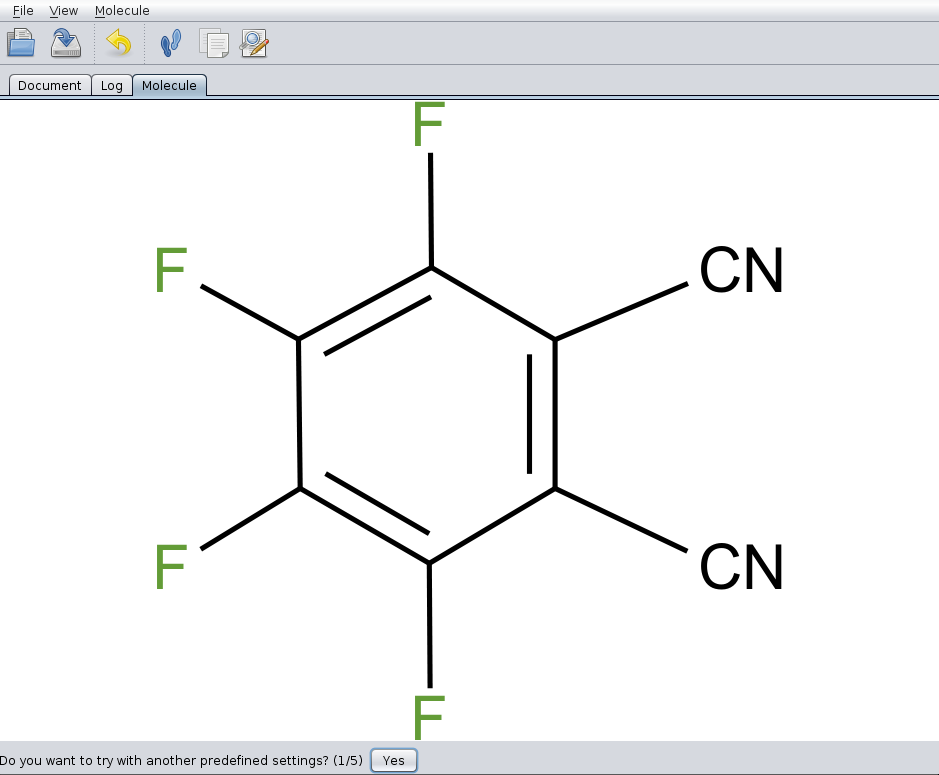
\includegraphics[scale=0.34]{media/demo.png}}
  \end{center}
\end{frame}

\begin{frame}
  \frametitle{Введение}
  \framesubtitle{Возникновение задачи: пополнение баз знаний}
  Соединение не так интересно само по себе. Интересен контекст.
  \begin{center}
     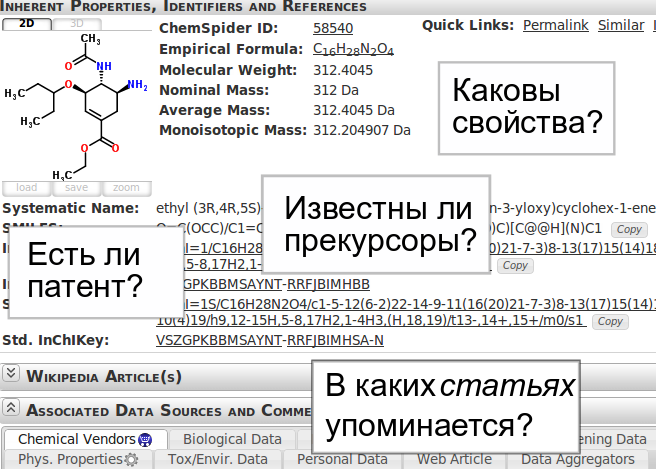
\includegraphics[scale=0.4]{media/chemspider.png}
  \end{center}
\end{frame}

\section{Распознавание}

\begin{frame}
  \frametitle{Распознавание}
  Этапы:
  \begin{enumerate}
    \item Обработка изображения
    \item Разбор изображения
    \item Извлечение связных компонент
    \item Отделение символьных компонент от графических
    \item Извлечение графа
      \begin{itemize}
        \item Кусочно-линейные элементы 
        \item Стереосвязи
        \item Кольца
      \end{itemize}
    \item Распознавание символов
    \item Объединение результатов
    \item Исправление химических ошибок
  \end{enumerate}
\end{frame}

\section{Этапы распознавания}
\subsection{Обработка изображения}

\begin{frame}
  \frametitle{Этапы распознавания}
  \framesubtitle{Обработка изображения}
  \begin{columns}
      \begin{column}{0.5\textwidth}
         Призвана облегчить последующие этапы 
        \begin{itemize}
         \item Фильтрация
         \item Бинаризация: перевод полутонового изображения в двуцветное
         \end{itemize}
      \end{column}
      \begin{column}{0.5\textwidth}
      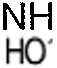
\includegraphics[scale=2.5]{media/bad.png}
      \end{column}
   \end{columns}
\end{frame}

\subsection{Разбор изображения}

\begin{frame}
   \frametitle{Этапы распознавания}
   \framesubtitle{Разбор изображения}
   \begin{columns}
     \begin{column}{0.4\textwidth}
      Изображение может быть сложным
      \begin{itemize}
        \item Таблицы заместителей
        \item Стрелки реакций
        \item Несколько молекул
      \end{itemize}
 \end{column}
 \begin{column}{0.6\textwidth}
   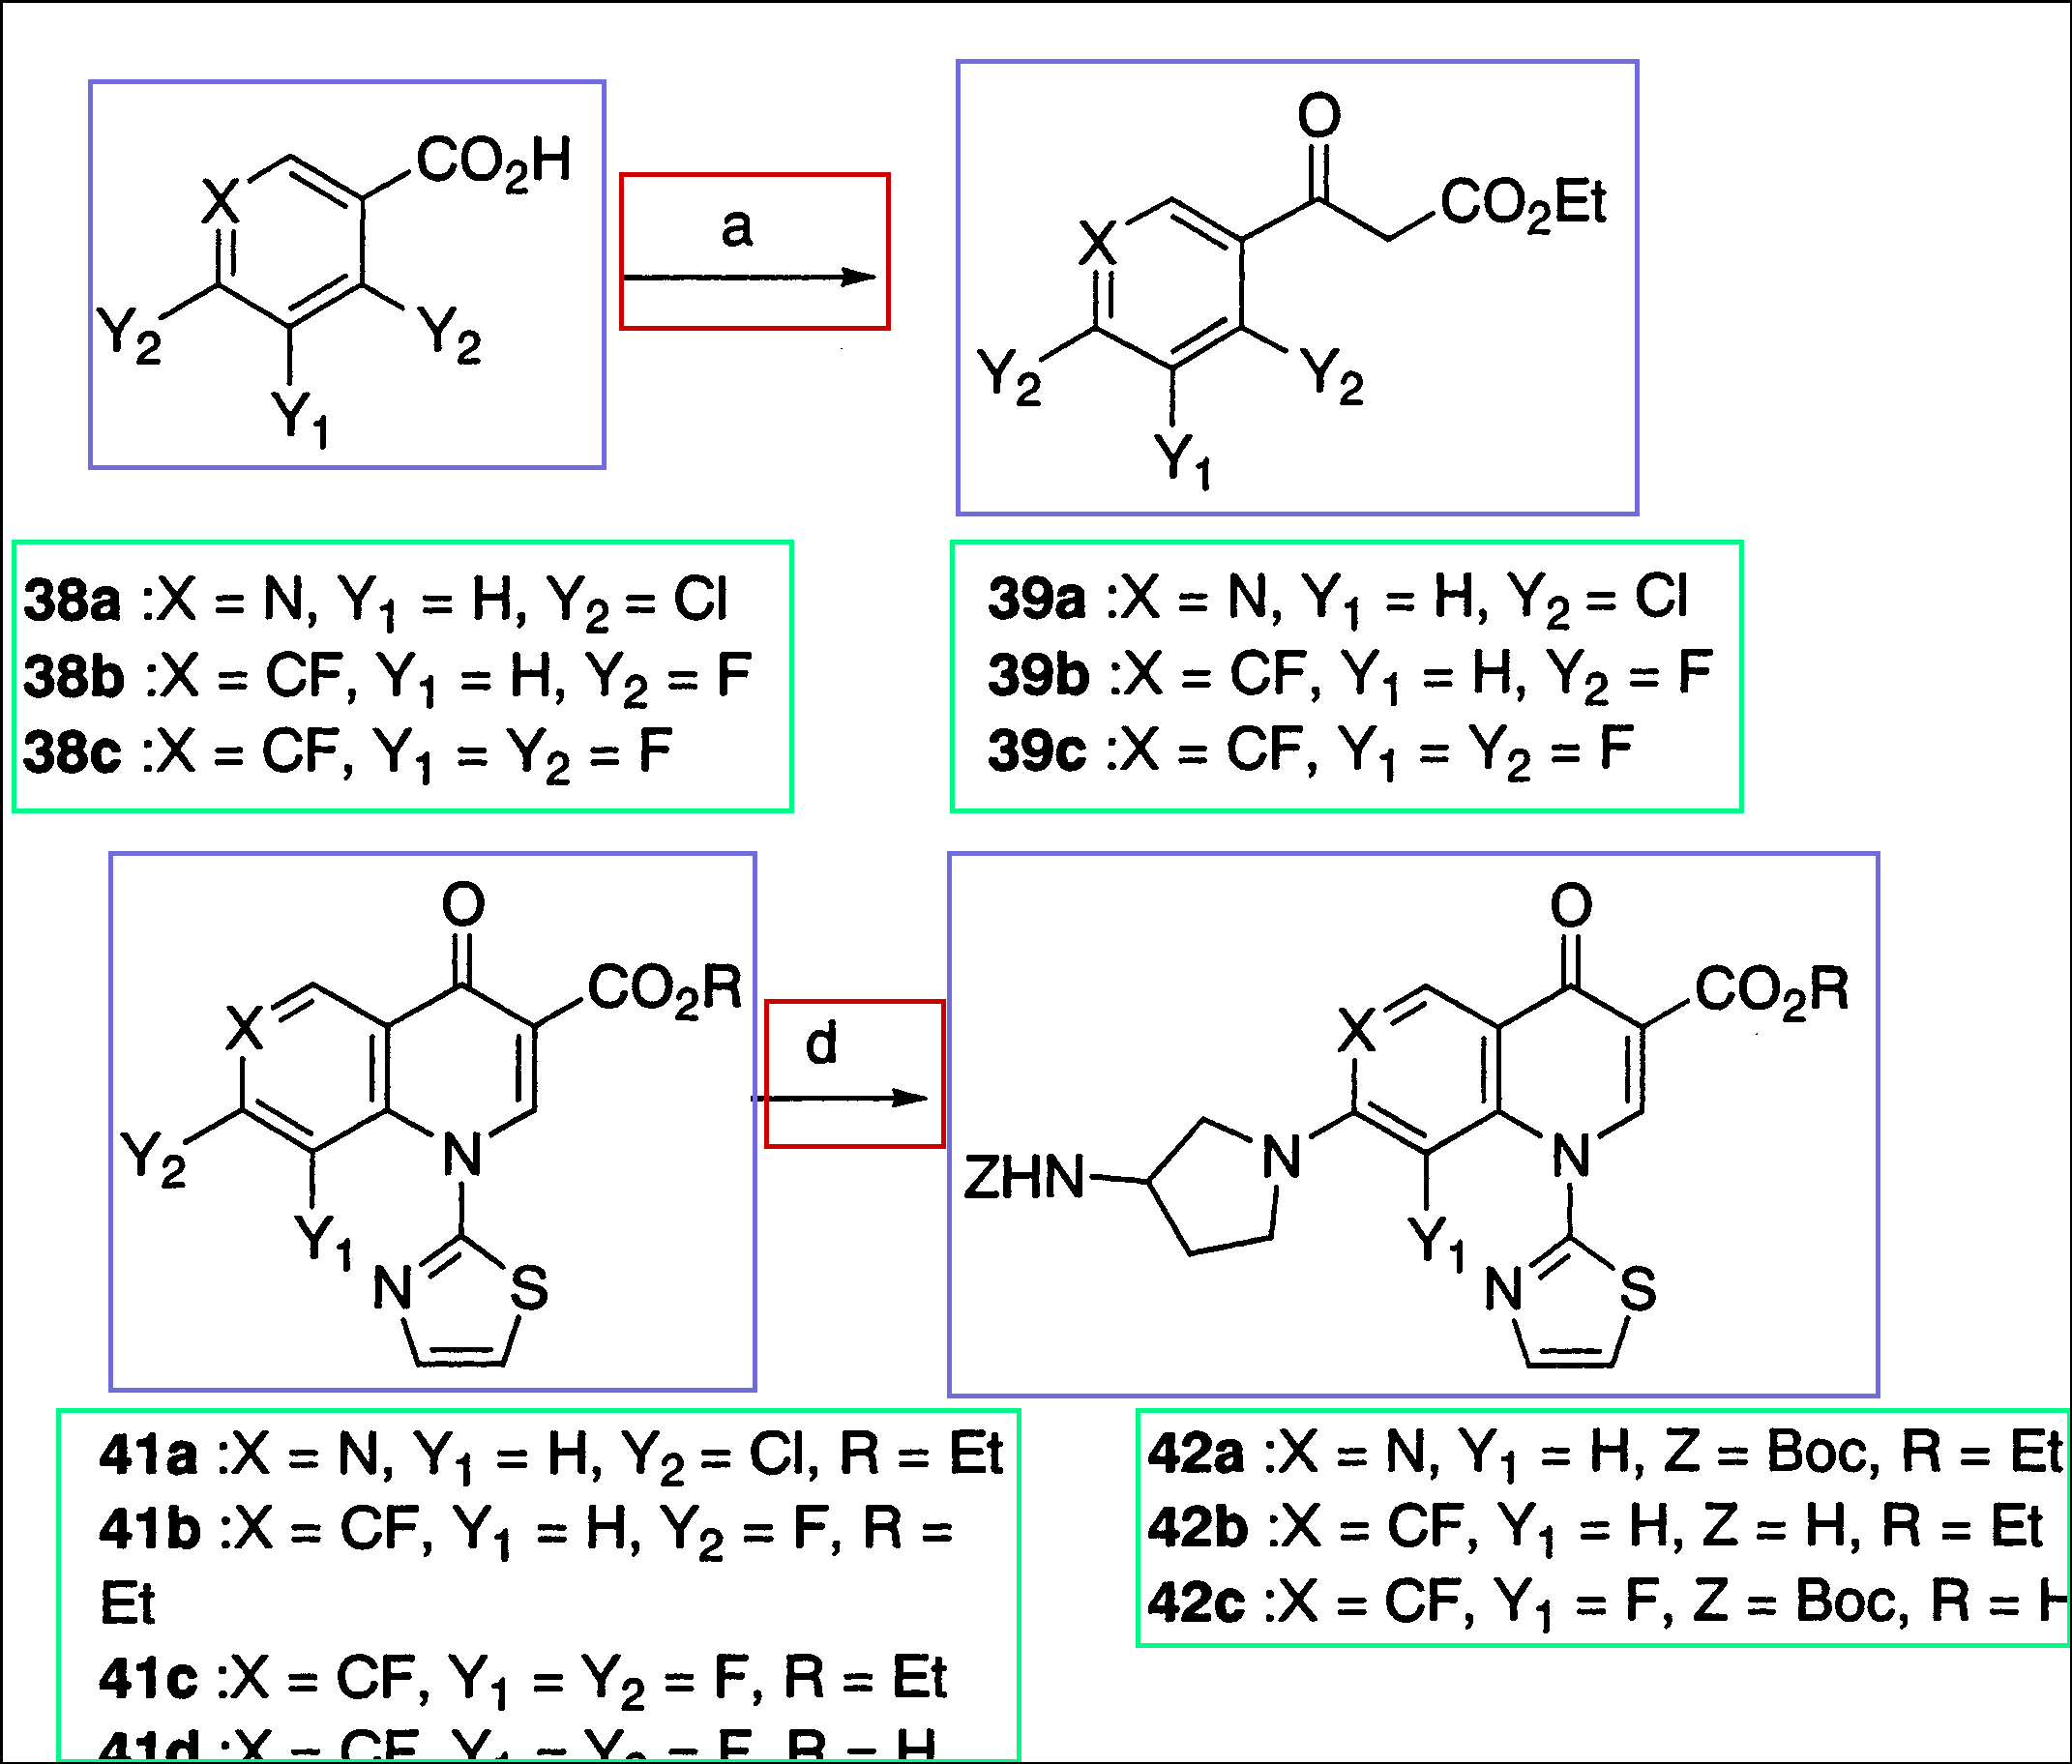
\includegraphics[scale=0.4]{media/superseg.png}
 \end{column}
 \end{columns}
\end{frame}

\subsection{Сегментация}

\begin{frame}
  \frametitle{Этапы распознавания}
  \framesubtitle{Сегментация. Разделение на компоненты связности}
  \begin{center}
  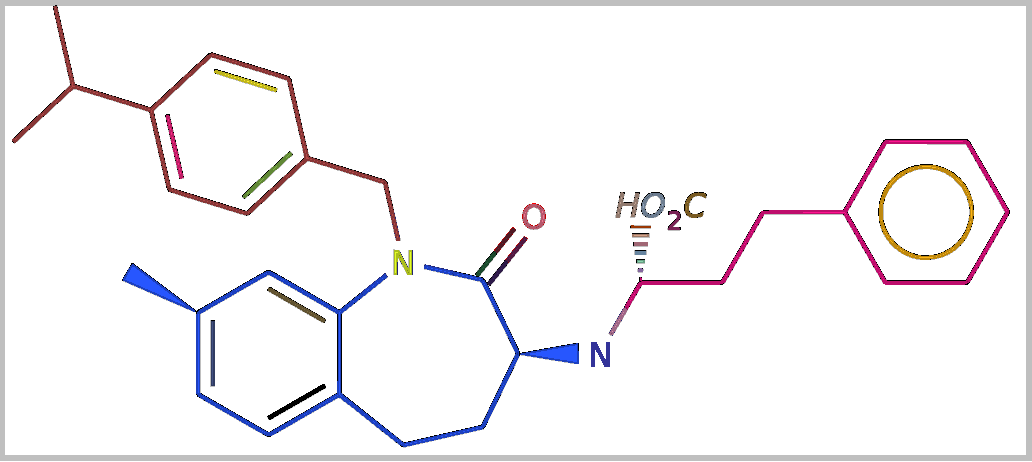
\includegraphics[scale=0.7]{media/mol_begin.pdf}
\end{center}

\end{frame}

\subsection{Символьная и графическая информация}

\begin{frame}
  \frametitle{Этапы распознавания}
  \framesubtitle{Символьная и графическая информация}
  Разделение происходит на основе оценки высоты заглавного символа и различных эвристик
  \begin{center}
  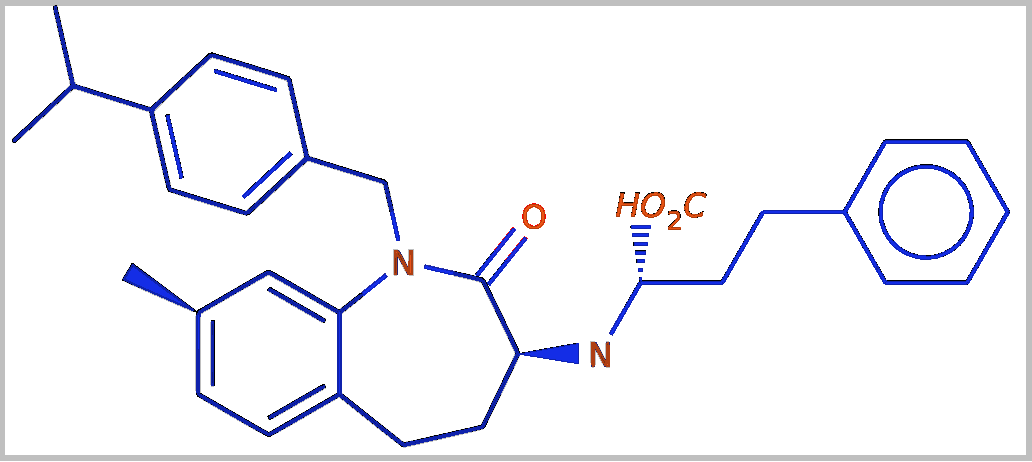
\includegraphics[scale=0.7]{media/mol2.pdf}
  \end{center}
\end{frame}

\subsection{Извлечение графа}

\begin{frame}
  \frametitle{Этапы распознавания}
  \framesubtitle{Извлечение графа: кусочно-линейные элементы}
  Картинка подвергается обработке фильтром утоньшения, а затем векторизации
  \begin{center}
  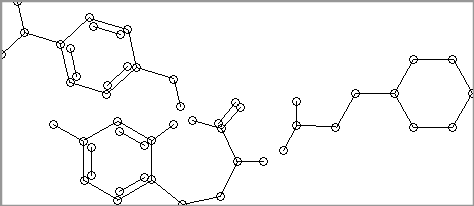
\includegraphics[scale=0.7]{media/ggg1.png}
  \end{center}
\end{frame}

\begin{frame}
  \frametitle{Этапы распознавания}
  \framesubtitle{Извлечение графа: кольца и стереосвязи}
  \begin{columns}
    \begin{column}{0.5\textwidth}
      \begin{itemize}
        \item Распознавание стерео-вверх связей происходит после векторизации с помощью анализа толщины связи 
      \end{itemize}
    \end{column}
    \begin{column}{0.5\textwidth}
      \begin{itemize}
        \item Кольца распознаются с помощью анализа дескрипторов контура сегмента
      \end{itemize}
    \end{column}
  \end{columns}
  \begin{center}
  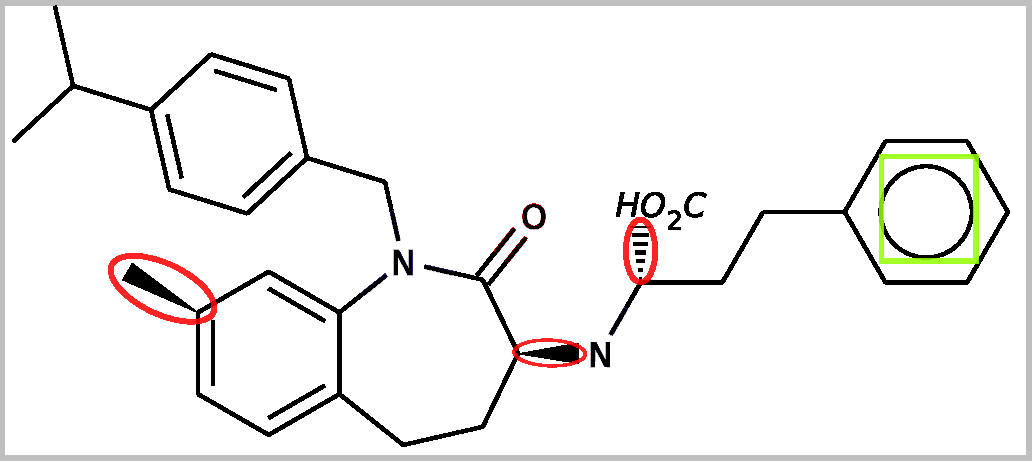
\includegraphics[scale=0.7]{media/mol3.pdf}
  \end{center}
\end{frame}

\subsection{Распознавание символов}

\begin{frame}
  \frametitle{Этапы распознавания}
  \framesubtitle{Распознавание символов}

  \begin{columns}
    \begin{column}{0.62\textwidth}
   \begin{enumerate}
    \item Получение контура обходом в глубину в специальном графе
    \item Подсчет для контура дескрипторов Фурье
      \[
  a_n = -\frac{1}{n\pi}\sum_{k=1}^{m}\bigtriangleup\phi_k\sin(\frac{2\pi n l_k}{L}) \] \\~
\[  b_n = \frac{1}{n\pi}\sum_{k=1}^{m}\bigtriangleup\phi_k\cos(\frac{2\pi n l_k}{L})
\]
    \item Сравнение дескрипторов c эталонными
   \end{enumerate}
   \end{column}
   \begin{column}{0.4\textwidth}
\centering     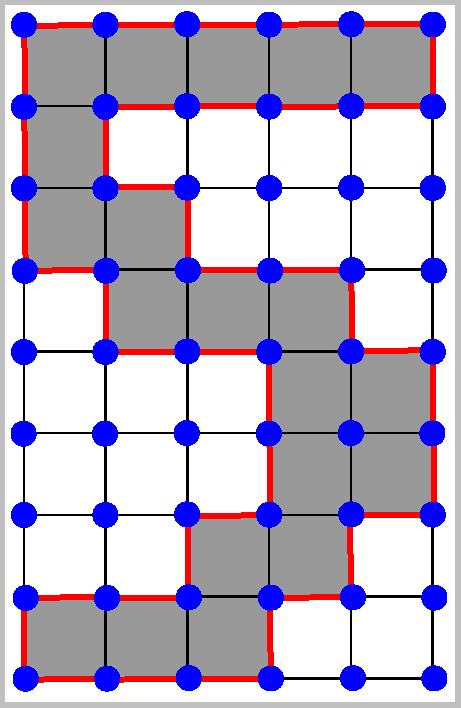
\includegraphics[scale=0.4]{media/five.pdf}
   \end{column}
 \end{columns}
\end{frame}

\subsection{Сборка молекулы и дополнение химической информацией}

\begin{frame}
  \frametitle{Этапы распознавания}
  \framesubtitle{Объединение результатов и дополнение химической информацией}
  Построение молекулярного графа:
  \begin{itemize}
    \item Поиск и объединение кратных связей
    \item Объединение близких вершин
    \item Закрепление меток атомов
  \end{itemize}
  Дополнения:
  \begin{columns}
    \begin{column}{0.5\textwidth}
  \begin{itemize}
    \item Ароматизация связей вокруг кольца
    \item Исправление неправильных направлений стереосвязей
  \end{itemize}
\end{column}
\begin{column}{0.5\textwidth}
    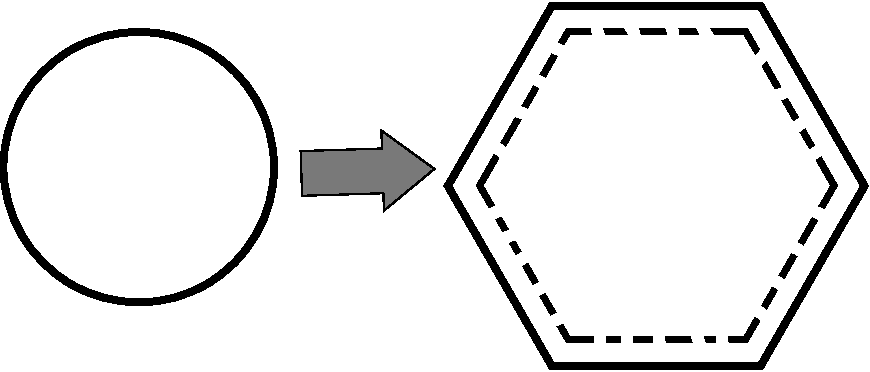
\includegraphics[scale=0.3]{media/aromatic.pdf}
\end{column}
\end{columns}
\end{frame}

\subsection{Результаты}

\begin{frame}
  \frametitle{Результаты}
  Уже существуют несколько наборов изображений и соответствующих файлов с машинным представлением для испытаний

  \begin{columns}
    \begin{column}{0.5\textwidth}
      \begin{center}\emph{USPTO \footnotemark} \\ 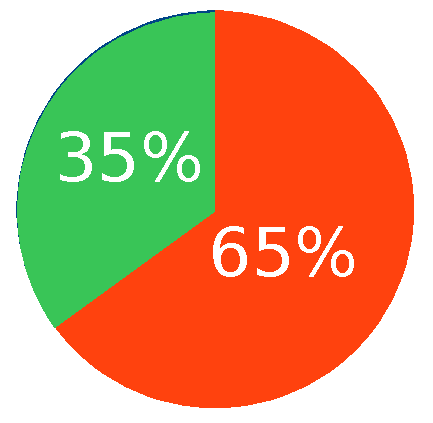
\includegraphics[scale=0.45]{media/pie_chart2.pdf} \\ 5700 изображений \\
      $\sim$10минут \\ $\sim$1.4 секунды на изображение \end{center}
    \end{column}
    \begin{column}{0.5\textwidth}
      \begin{center}\emph{Chem-Infty} \\ 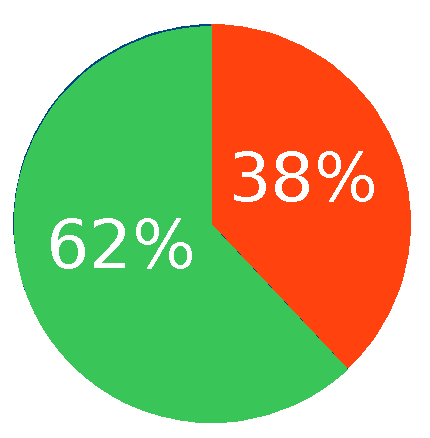
\includegraphics[scale=0.4]{media/pie_chart1.pdf} \\ 
        450 изображений \\ $\sim$10 минут \\ $\sim$1.3 секунды на изображение  \end{center}
    \end{column}
  \end{columns}
  \footnotetext{United States Patent and Trademark Office}
\end{frame}

\section{Алгоритмы}

\begin{frame}
  \frametitle{Алгоритмы}

  Известные

  \begin{enumerate}
    \item Фильтрация. Свертка изображения с различными ядрами.
    \item Утоньшение \\ 
      Joseph M. Cychosz, \emph{Efficient Binary Image Thinning using Neighborhood Maps}, Graphics Gems IV, Academic Press, 1994
    \item Распознавание символов \\
      Charles T. Zahn \& Ralph Z. Roskies,
  \emph{Fourier Descriptors for Plane Closed Curves},
   IEEE Transactions on computers, Vol. c-21, No. 3, march 1972
  \end{enumerate}
      
  Оригинальные

  \begin{enumerate}
    \item Разделение символьной и графической информации
    \item Извлечение кусочно-линейных элементов
  \end{enumerate}
\end{frame}

\section{Планы на будущее}

\begin{frame}
  \frametitle{Планы на будущее}
  \begin{itemize}
    \item Более сложная обработка изображения
    \item Учет дополнительной информации на картинке (таблицы заместителей, реакции)
    \item Раскрытие групп
    \item Интеллектуальный разбор изображения
    \item Контекстный анализ на основе известных из химии фактов
    \item Комплексный анализ документа
    \item Адаптция к работе с рукописными молекулам
    \item Улучшение качества распознавания
  \end{itemize}
\end{frame}

\section{Заключение}

\begin{frame}
  \frametitle{Заключение}
  \begin{columns}
    \begin{column}{0.7\textwidth}
  \begin{itemize}
    \item Задача актуальна и требует решения
    \item Существует большое количество сложных подзадач
      \begin{itemize}
        \item Слипшиеся связи и символы
        \item Связи, изображаемые кривыми
        \item Обобщенные молекулы
      \end{itemize}
  \end{itemize}
\centering  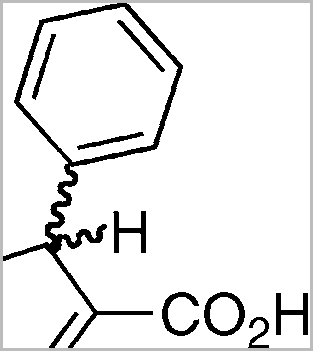
\includegraphics[scale=0.2]{media/complex3.png} 
  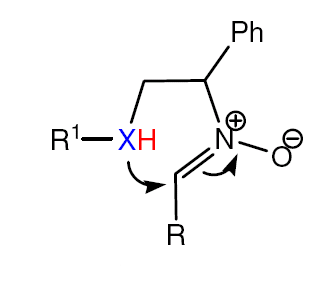
\includegraphics[scale=0.5]{media/complex.png}
\end{column}
\begin{column}{0.5\textwidth}
  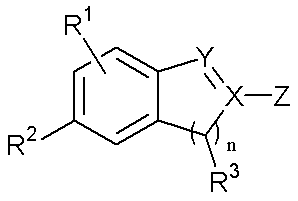
\includegraphics[scale=0.5]{media/Markush.png} \\
  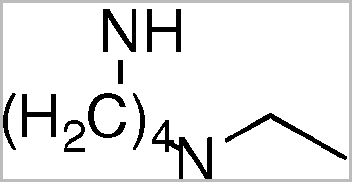
\includegraphics[scale=0.3]{media/complex2.png} \\
\end{column}
\end{columns}
\end{frame}

\begin{frame}
   \begin{center}
     \LARGEСпасибо за внимание! \\ 
     \url{http://scitouch.net/imago}
   \end{center}
\end{frame}

\end{document}
